\documentclass[conference]{IEEEtran}
\IEEEoverridecommandlockouts
% The preceding line is only needed to identify funding in the first footnote. If that is unneeded, please comment it out.
\usepackage{cite}
\usepackage{amsmath,amssymb,amsfonts}
\usepackage{algorithmic}
\usepackage{graphicx}
\usepackage{textcomp}
\usepackage{subfigure}
\usepackage{caption}

\def\BibTeX{{\rm B\kern-.05em{\sc i\kern-.025em b}\kern-.08em
    T\kern-.1667em\lower.7ex\hbox{E}\kern-.125emX}}

\newcommand{\tabincell}[2]{\begin{tabular}{@{}#1@{}}#2\end{tabular}}
    
\begin{document}

\title{A Fusion Method based on Multi-Dimensional Features for Insider Threat Detection\\
{\footnotesize \textsuperscript{*}Note: Sub-titles are not captured in Xplore and
should not be used}
\thanks{Identify applicable funding agency here. If none, delete this.}
}

\author{\IEEEauthorblockN{1\textsuperscript{st} Given Name Surname}
\IEEEauthorblockA{\textit{dept. name of organization (of Aff.)} \\
\textit{name of organization (of Aff.)}\\
City, Country \\
email address}
\and
\IEEEauthorblockN{2\textsuperscript{nd} Given Name Surname}
\IEEEauthorblockA{\textit{dept. name of organization (of Aff.)} \\
\textit{name of organization (of Aff.)}\\
City, Country \\
email address}

}

\maketitle

\begin{abstract}
While most security projects have focused on fending off attacks coming from outside the organizational boundaries, a real threat has arisen from the people who are inside those perimeter protections. Insider threats have shown their power by hugely affecting national security, financial stability, and the privacy of many thousands of people. What is in the news is the tip of the iceberg, with much more going on under the radar, and some threats never being detected.We propose two anomaly detection methods.The first method seeks to identify anomalous behavior that blends within each information source.The second method identifies unusual changes in behavior over time using a Markov model approach. Finally, we present a fusion approach that integrates evidence from both methods to improve the accuracy and robustness of the insider threat detection system. 
\end{abstract}

\begin{IEEEkeywords}
anomaly detection, insider threat detection, information fusion, machine learning
\end{IEEEkeywords}

\section{Introduction}

Insider threat, or the threat from a malicious insider who is defined as ``a current or former employee, contractor or business partner who has, or had, authorized access to an organization’s network, system or data and intentionally exceeded or misused that access in a manner that negatively affected the confidentiality, integrity or availability of the organization’s information or information systems''  \cite{b1} has been identified as a primary concern within the cybersecurity community. Financial loss and reputation damage caused by this ``known unknow'' cybersecurity threat far outweighs that caused by external attacks. The Breach Level Index, which tracks publicly disclosed breaches, shows that almost 40\% of data breaches are attributed to malicious insiders or accidental loss due to insiders\cite{b2}.Thus Insider threat activities pose a severe challenge to the well-being of an organization, and it is naturally critical for organizations to guard against such events.

One of the most recent articles from CSO magazine\cite{b3} compared the cost between external and internal attacks and noted that while it takes about 50 days to fix a data breach caused by an internal attack, it only takes 2 to 5 days in the case of external attacks. Moreover, “attacks by malicious insiders are also the costliest to fix (\$145,000), followed by denial of service (\$127,000) and Web-based attacks (\$96,000)”, indicating the severity of this problem.

For these reasons the insider threat detection problem has been studied extensively\cite{b4}. This includes work done in the cyber-security realm, social science, governmental organizations and other relevant filed. In comparison with the traditional approaches of post attack analysis and subsequent change of policy, detecting threats from data offers the benefit of continuous and in time evaluation. Methods based data analytics include the work done by Mathew et al.\cite{b5} on account of user access patterns, the work of Eberle et al. \cite{b6} on using social graphs to detecting the abnormal.There have also been various approaches based on specific insider threat scenarios to detect abnormal\cite{b7}\cite{b8}. However ,the unpredictable nature of human behavior makes this complex issue much more complicated than expected. This is aggravated by the mobility and hyperconnectivity of people. Insider threat research and surveys suggest this problem cannot be considered only as a data driven problem; it needs to be considered as data and behavior driven problem \cite{b9}.A close analysis of user behavior can spot trends and such information can be used in tightening radars on suspicious users. There are several papers based on behavioral models\cite{b10}\cite{b11}\cite{b12}. Hoda et al. \cite{b13}detect peer groups of users and modeling user behavior with respect to these peer groups, and subsequently detect insider activity by identifying users who deviate from their peers with respect to the user behavior models. Although some methods based on fusion of multi-source information and user behavior\cite{b14}, they got low accuracy due to the difficulty of insider threat detection. Sean Robinson et al.\cite{b15} used deep learning to improve the accuracy with the cost of the complexity of the algorithm.

Consideration of above facts led us to propose a fusion method based on multi-dimensional features that simultaneously processes the heterogeneous information sources and fuses the processed output to detect anomalies in a more robust and accurate manner. The proposed architecture detects anomalous behavior from multi-source information based on data-driven and time series dimensions based on user behavior modeling with low algorithm complexity and high accuracy. It has three major components “Across-Domain Anomaly Detection(ADAD)” , “Across-Time Anomaly Detection(ATAD)” and “Information Fusion for Combining Anomaly Indicators (ADAD)”. The multidimensional data from the enterprise network is formatted and fed separately into the MDCV and ATAD, which generates an abnormal score representing the users unusual behavior. These input streams can come from heterogeneous sources of information in different data formats. And then we get the final abnormal score based on different dimensions through the IFCAI by fusion the abnormal scores  for abnormal detection.

\begin{figure*}[htb]
\centerline{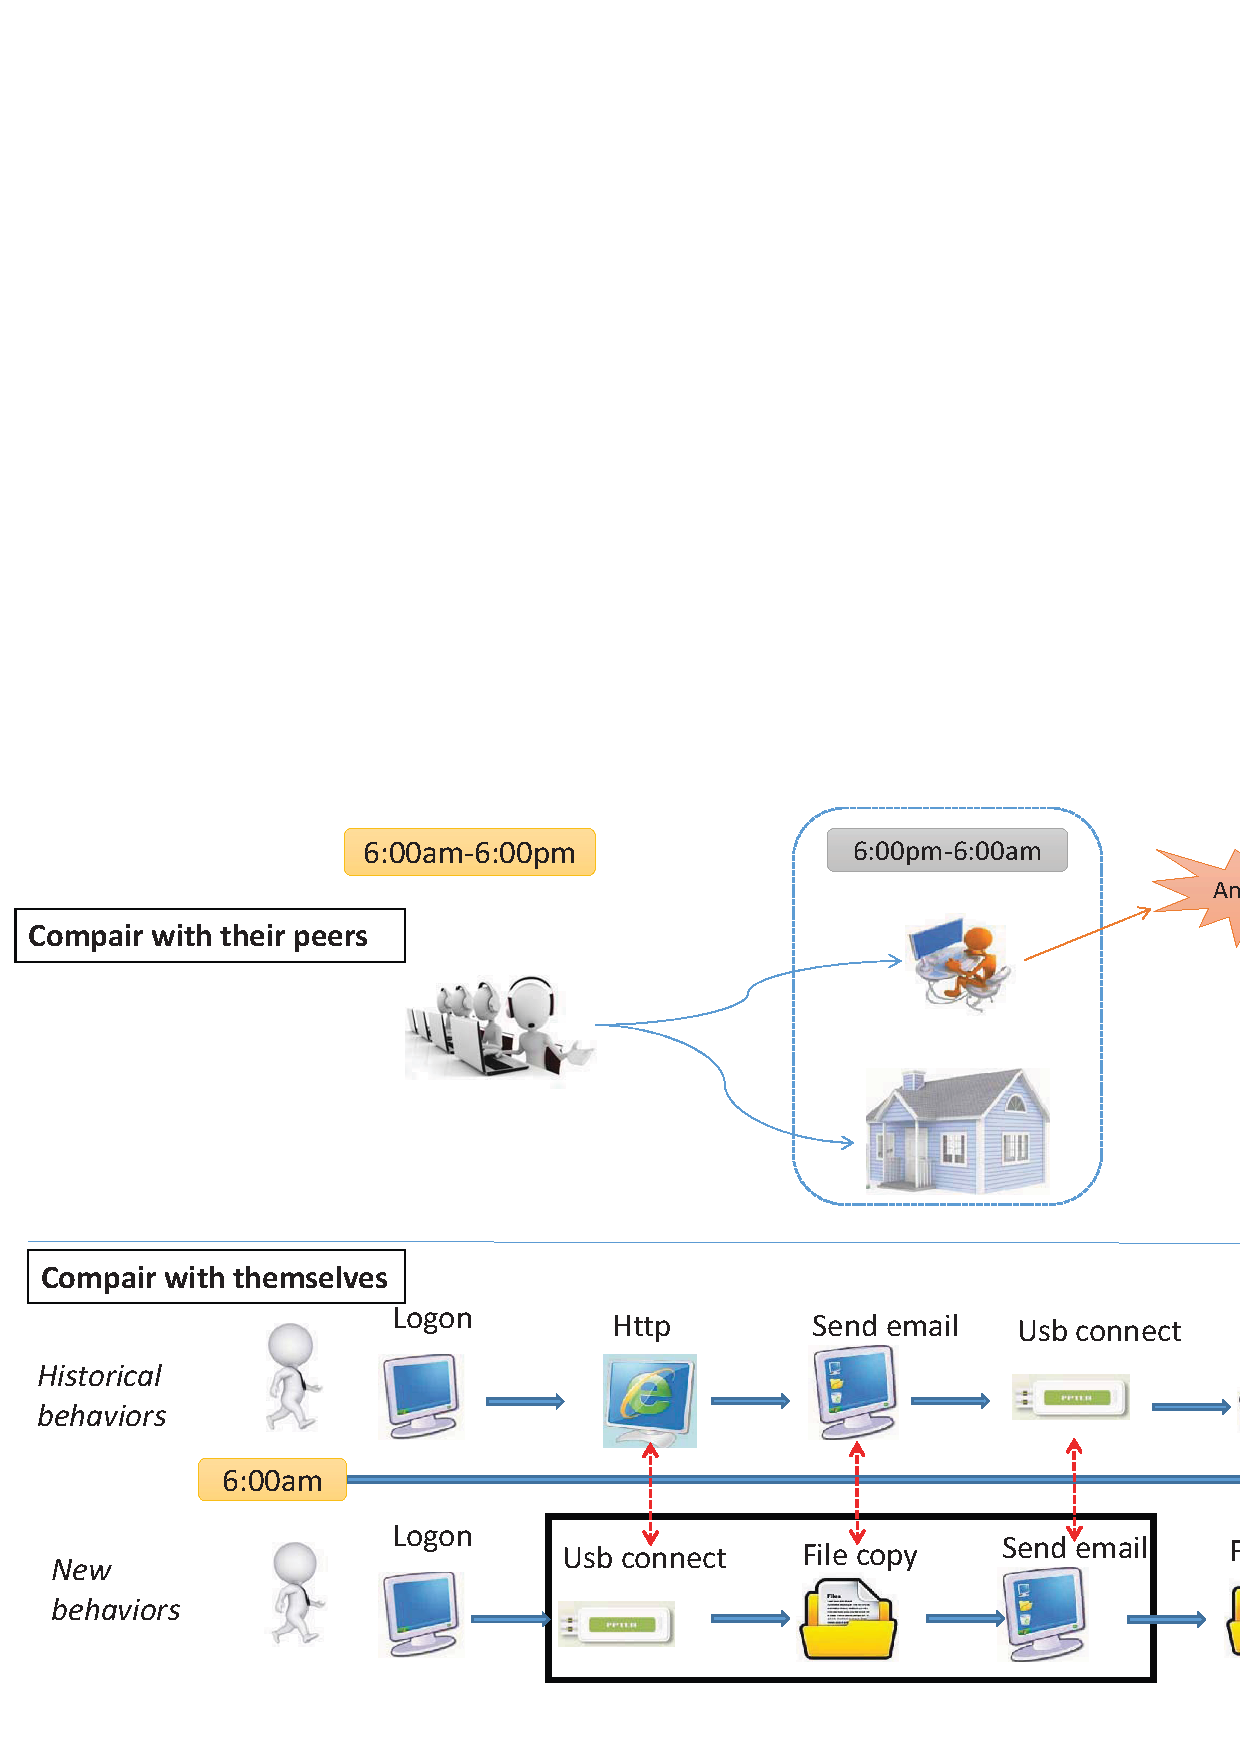
\includegraphics[width = 0.8\textwidth]{figure/figure1.png}}
\caption{Example of insider threat.}
\label{fig}
\end{figure*}


\section{Related work}


The topic of insider threat has attracted much attention recently in different fields. Researchers have proposed different models aimed at preventing or detecting the presence of attacks (e.g., \cite{b16}and \cite{b17}). There is much work that in consideration of the psychological and behavioral characteristics of insiders who may pose a threat as means for detection (e.g., \cite{b18}–\cite{b19}). Kammüller and Probst \cite{b20} considered how organizations can identify attack media according to policy irregularities, to minimize the potential of insider attacks. Similarly, Ogiela and Ogiela \cite{b21} studied how to use hierarchical and threshold secret sharing to prevent insider threats. 

Early work by Magklaras and Furnell\cite{b22} considers how to estimate the level of threat that is likely to originate from a particular insider based on certain profiles of user behavior. As they acknowledge, substantial work is still required to validate the proposed solutions.

Early work by Spitzner \cite{b23} discusses the use of honeypots (decoy machines that may lure an attack) for detecting insider attacks. However, as security awareness increases, those choosing to commit insider attacks are finding more subtle methods to cause harm or defraud their organizations, and thus, there is a need for more sophisticated prevention and detection. Early work by Magklaras and Furnell \cite{b24} considers how to estimate the level of threat that is likely to originate from a particular insider based on certain profiles of user behavior. As they acknowledge, substantial work is still required to validate the proposed solutions. Myers et al.\cite{b25}  considered how web server log data can be used to identify malicious insiders who look to exploit internal systems. Maloof and Stephens \cite{b26} proposed a detection tool for when insiders violate need-toknow restrictions that are in place within the organization. Okolica et al. \cite{b27} used probabilistic latent semantic indexing with users to determine employee interests, which are used to form social graphs that can highlight insiders. Liu et al. \cite{b28} proposed a multilevel framework, which is called sensitive information dissemination detection, that incorporates networklevel application identification, content signature generation and detection, and covert communication detection.

More recently, Eldardiry et al. \cite{b29} have also proposed a system for insider threat detection based on feature extraction from user activities. However, they did not factor in the change of user behavior over time. We note that while a common activity not be suspicious, a rare change of the order  common activity can be. In this paper we propose a method to detects individuals that considers not only the features from user activity but also the change of the activity over time. Brdiczka et al.  \cite{b30}combined psychological profiling with structural anomaly detection to develop an architecture for insider threat detection. They used data collected from the multiplayer online game, i.e., World of Warcraft, to predict whether a player will quit their guild. In contrast to real-world insider threat detection, they acknowledged that the game contains obvious malicious behaviors; however, they aimed to apply these techniques to real-world enterprises. Eberle et al. \cite{b31} considered graph-based anomaly detection as a tool for detecting insiders, based on modifications, insertions, and deletions of activities from the graph. They used the Enron e-mail data set \cite{b32} and cellphone traffic as two preliminary cases, within the intention of extending to the CERT insider threat data sets. Senator et al. \cite{b33} proposed to combine structural and semantic information on user behavior to develop a real-world detection system. They used a real corporate database, gathered as part of the Anomaly Detection at Multiple Scales program; however, due to confidentiality, they cannot disclose the full details, and thus, it is difficult to compare against the work. Parveen et al. \cite{b34} used stream mining and graph mining to detect insider activity in large volumes of streaming data, based on ensemble-based methods, unsupervised learning, and graph-based anomaly detection. Parveen and Thuraisingham \cite{b35} extended the work with an incremental learning algorithm for insider threat detection that is based on maintaining repetitive sequences of events. They used trace files collected from real users of the Unix C shell \cite{b36} ; however, this public data set is relatively dated now. Tabish Rashid \cite{b37} takes the change of user behavior  over time to detect the anomaly,however,it has to pay algorithm complexity. Michael Goldsmith use some methods based on fusion of multi-source information and user behavior\cite{b38},however, they got a not optimistic accuracy due to the difficulty of insider threat detection.

One clear observation from these related work is that access to real-world data is extremely difficult, and thus, researchers synthesize data that are similar to that of a real-world enterprise, or use a subset of data points, or apply insider threat detection techniques to other problem domains (e.g., online games).

And in the part of the construction of the normal user portrait, most tend to find a normal portrait in all users behaviors in order to detect insider threat that does not meet this normal portrait. It will lead some of the special nature of the staff to be the error detection anomalies; or separate consideration of the abnormal changes in the behavior as the basis for detection, which will miss some of the true threat with abnormal behavior . Our approach combines these two factors from the comparison with the behavior of peers and their own historical behavior . As the figure1 shows, we use of the approach based on multi-domain feature fusion to detect the abnormal behavior between users and colleagues. For example, after get off work, the general behavior is that everyone will go home to rest, and some of the few people will choose to continue working after the work, even in the early hours will still deal with some of the company's sensitive information services. This is one of the abnormal scenarios we have taken into account. On the other hand, we use time series detection method to compare the user's current behavior and historical behavior to find the difference. For example, an employee's long-term behavior is to click on the browser after booting, and view the email then reply to a series of messages. But one day, he connected the mobile device after booting , and a series of operations on the file-copy, which does not match his usual style of doing things. And this series of operations is also sensitive to company's information. We can detect this unusual behavior of the user depending on this. Considering these two factors, we propose a method with high accuracy and low algorithm complexity, which is of great significance in industry and scientific research.

\section{Overview of proposed approach}

We propose a fusion method based on multi-dimensional features for insider threat detection which is illustrated in Figure 2. First, for multi-source information,we extract features in two dimensions,one we count and analyze the characteristics of each domain(e.g., logons),and the other we focus on time-series behaviors of user to identify changes in activities of a user compared to that user’s past activities.

After the features extraction, the architecture has two main components - one component for detecting abnormality across information sources (or domains) named “Across-Domain Anomaly Detection(ADAD)”, and another for detecting inconsistencies across time named “Across-Time Anomaly Detection(ATAD)” - which are then fused together to improve accuracy and robustness. These components are briefly described in next section.

\begin{figure}[htb]
\centerline{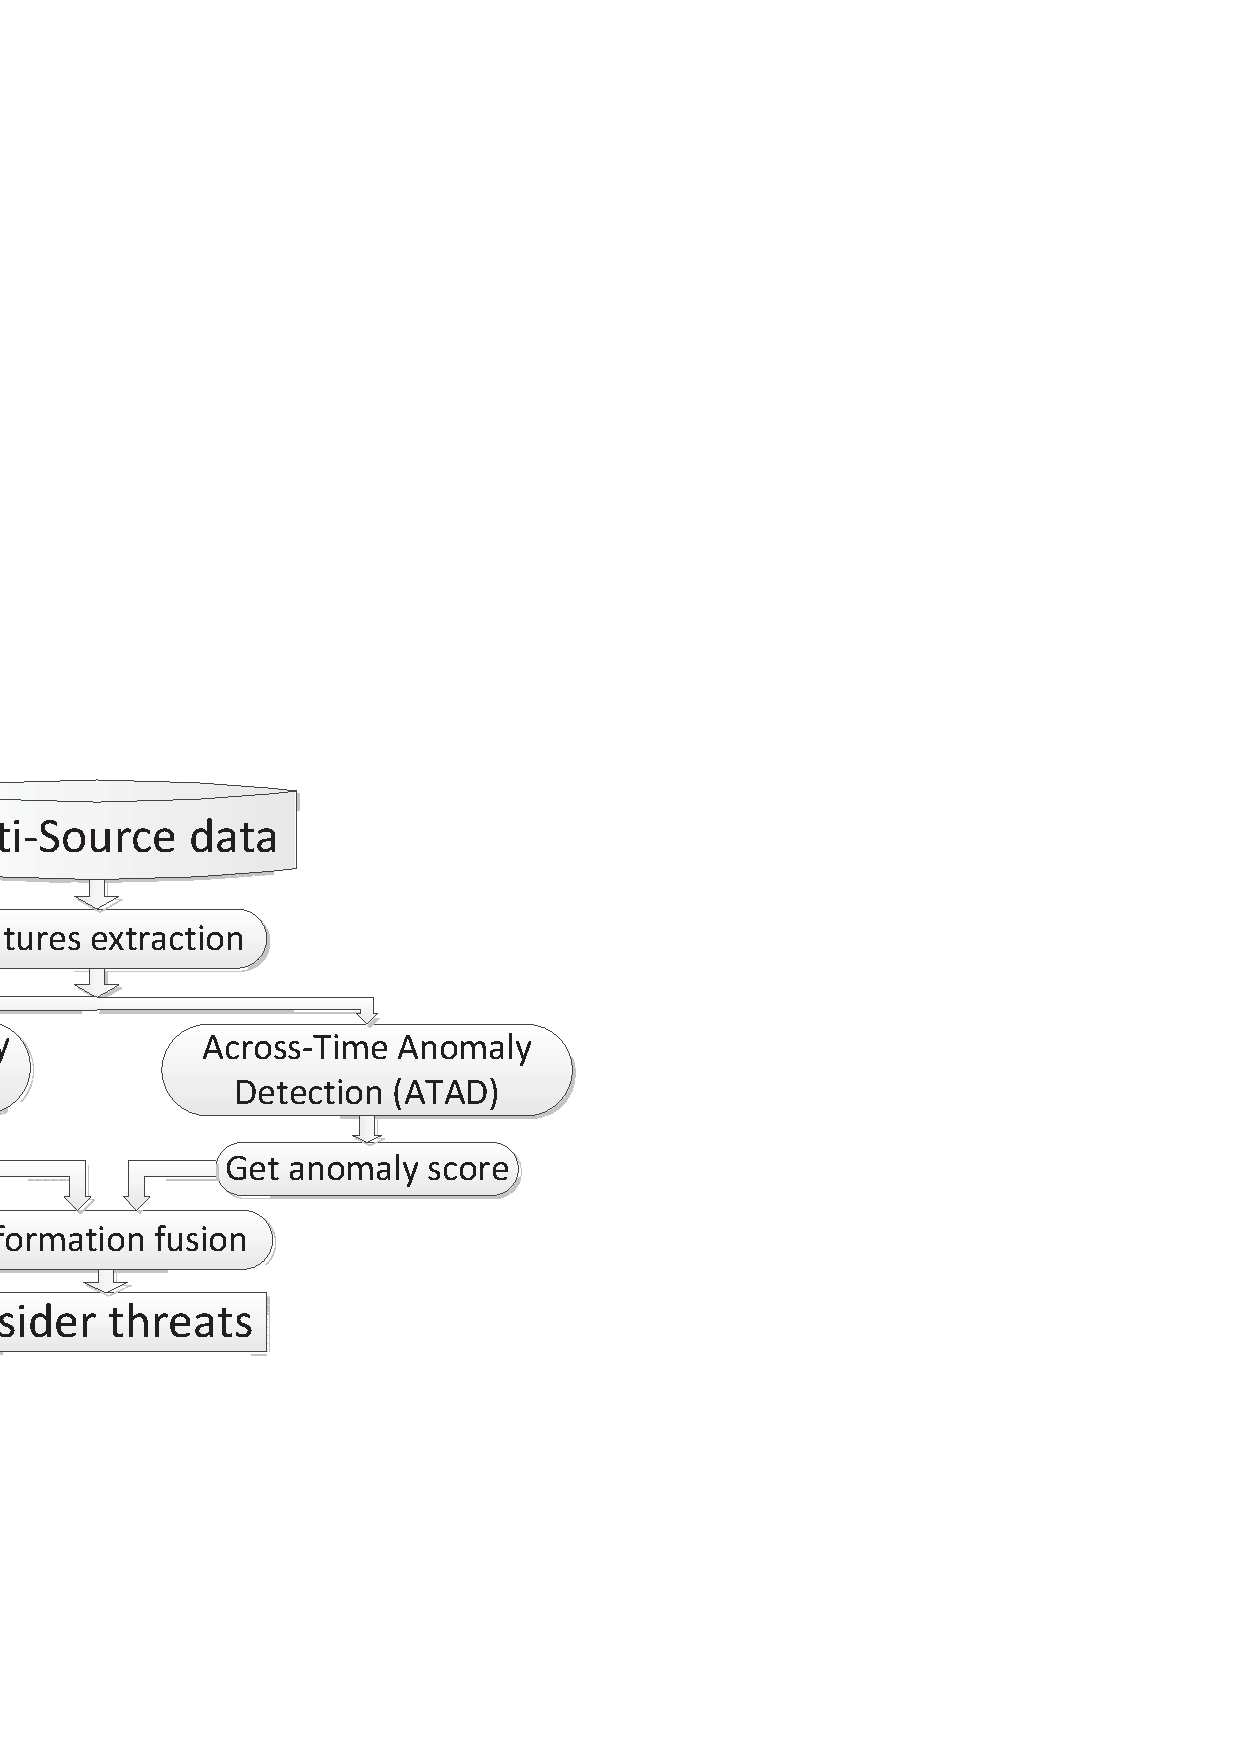
\includegraphics[width = 0.5\textwidth]{figure/figure2.png}}
\caption{Anomaly Detection Framework.}
\label{fig}
\end{figure}

\subsection{The Data Set}

Due to the lack of availability of proper insider threat datasets we have utilized the insider threat
dataset published by CERT Carnegie Mellon University for this research \cite{b39} The dataset “R4.2.tar.bz” has been used for this analysis. According to the dataset owners, this is a “dense needle” dataset with a fair amount of red team scenarios. This dataset consists of six broad types of data records (HTTP, logon, device, file, email and psychometric) of 1000 employees over a 17 months period. All HTTP records contain user, PC, URL and web page content with time stamps. “Logon.csv” consists of user logon/logoff activities with the corresponding PC with timestamps. “Logon” and “Logoff” are the two types of activities can be found in data records. “Logon” activity corresponds to either a user login event or a screen unlock event, while the “Logoff” event corresponds to user logoff event. Screen locks are not recorded in this dataset. The third data file “device.csv” is a collection of data records of removable media usage. It indicates insert/remove actions with the relevant user, PC, and timestamp. Details of file copies are stored in “file.csv” file with date, user, PC, filename, and content. To get the friendship network of users, the CERT dataset provides email communication records including from, to, cc and bcc fields. 


\section{APPROACH}


\subsection{Approach 1:Across-Domain Anomaly Detection(ADAD)}\label{AA}

We define the problem as follows. An anomalous user is one that exhibits inconsistent behavior across the domians. The intuition is that user activity should be reflect in any domain, and most users exhibit similar behavior within each domain.For example, most people would sleep at midnight, but few maybe login the system and do some business such as copying lots of files. This behavior different from most peers not only occur in a domain, but all domains. So  we believe that it is sufficient to consider all behaviors from every domain to characterize the user's behavior. The figure 2 is the structure of the approach.

\begin{figure}[htb]
\centerline{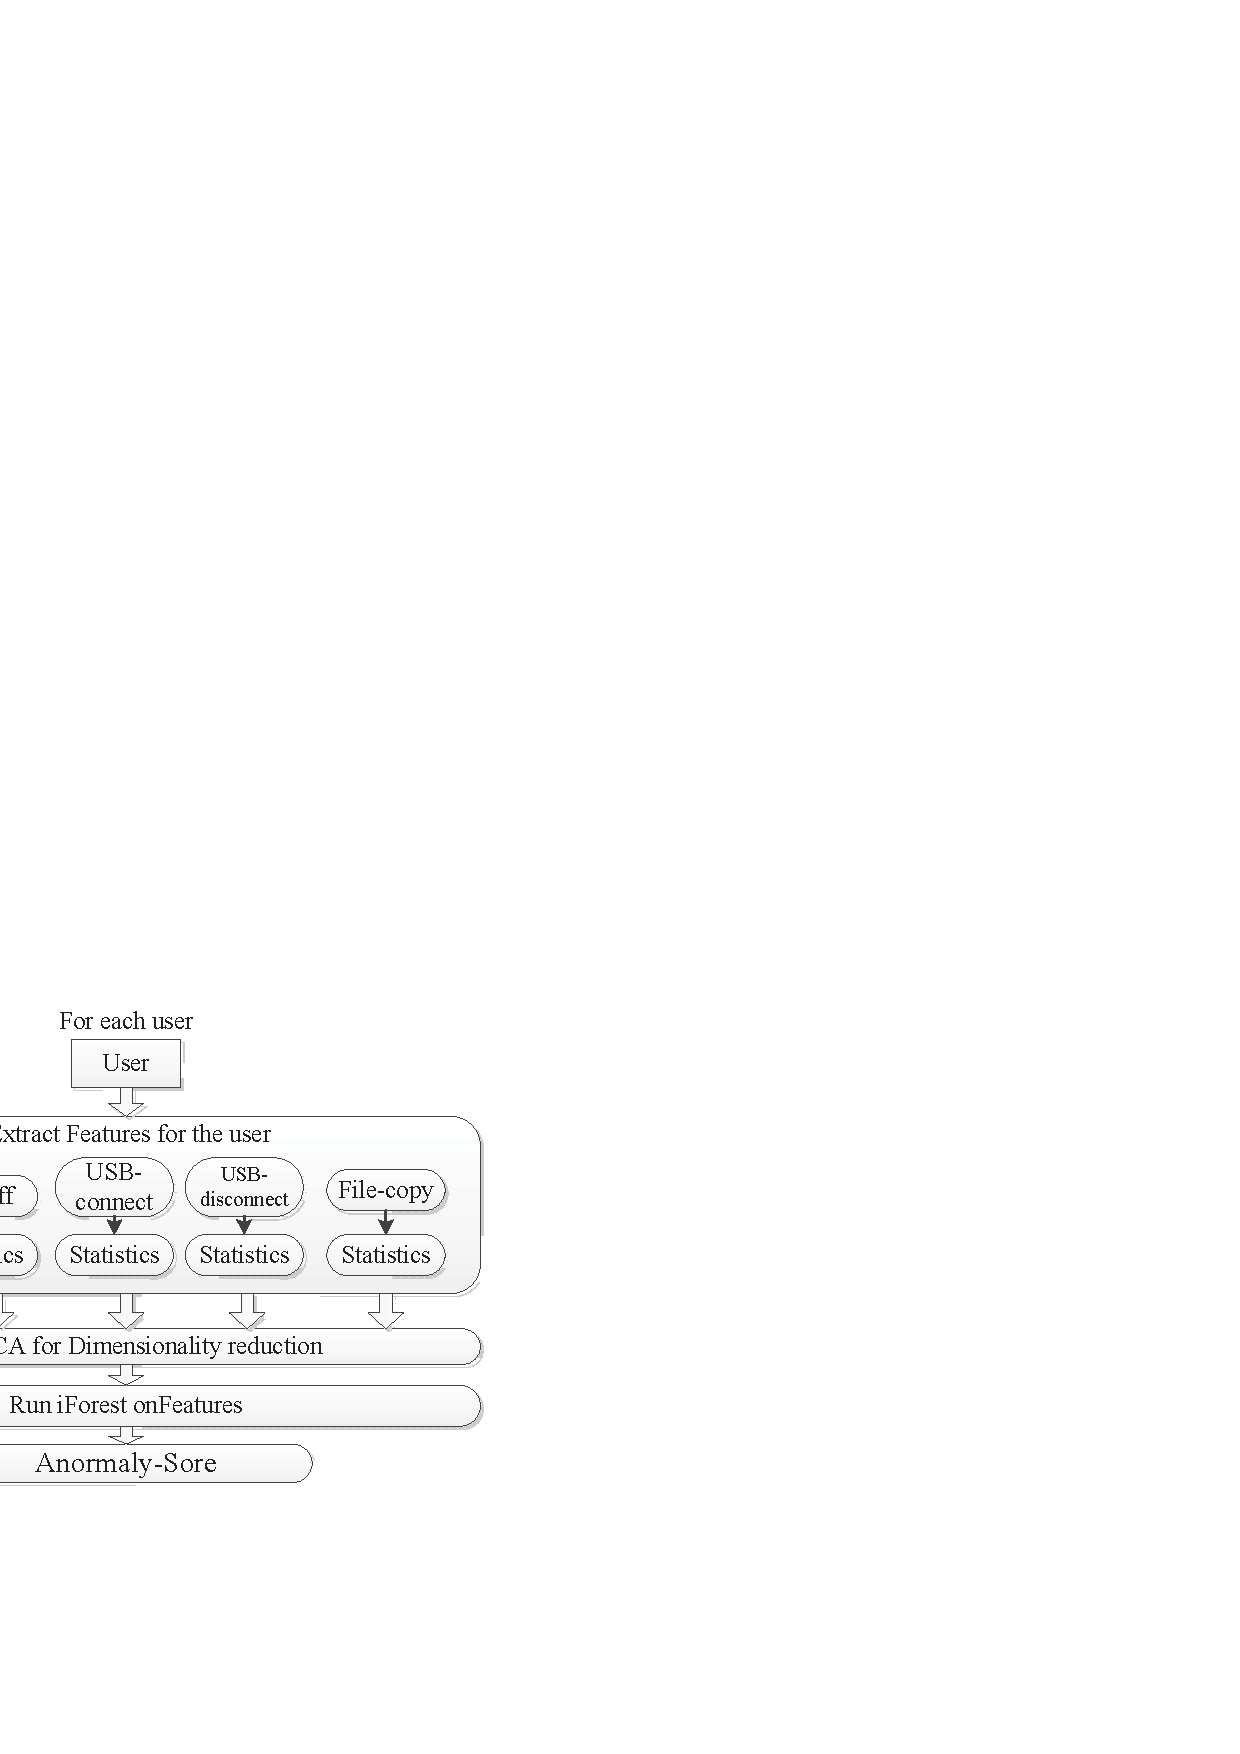
\includegraphics[width = 0.6\textwidth]{figure/figure3.png}}
\caption{An overview of the Across-Domain Anomaly Detection(ADAD).}
\label{fig}
\end{figure}

\subsubsection{Feature Extraction}

Individual logon logoff events. This parameter can be used in identifying users abnormal logon/logoff activities as most disgruntled insiders tend to commit malicious activities after hours \cite{b40}. Identifying users’ baseline behavior on system/device access is an essential part of malicious insider threat detection problem. For each user, four parameters (minimum, maximum, mean and mode) logon and logoff values have been calculated. 

\begin{figure*}[!t]
\centering
\subfigure[Logon behavior]{
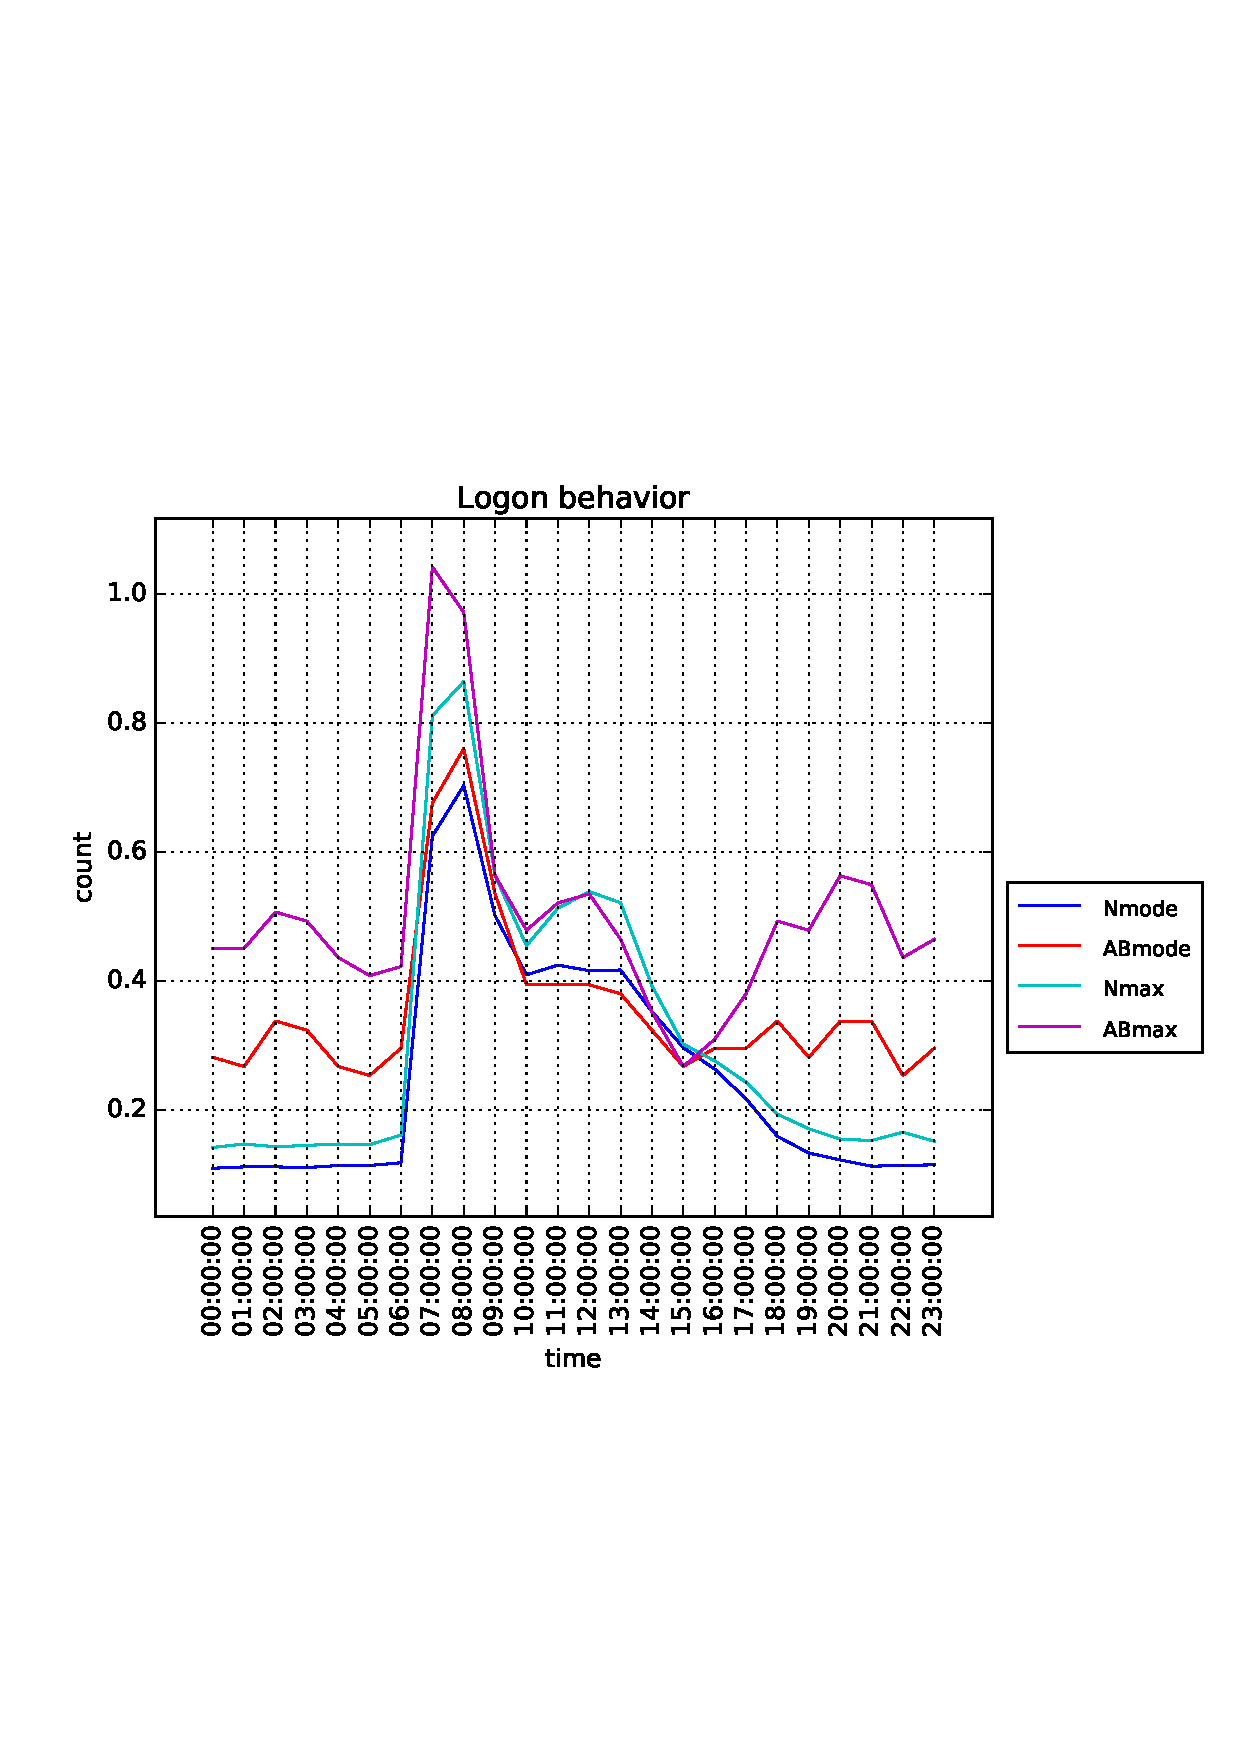
\includegraphics[width=2.8in]{figure/figure41.png}
} 
\subfigure[Logoff behavior]
{
 \includegraphics[width=2.8in]{figure/figure42.png}
}
\caption{ Users’ logon and logoff behavior }
\label{fig5}
\end{figure*}

\begin{figure*}[!t]
\centering
\subfigure[USB connect]{
\includegraphics[width=2.8in]{figure/figure51.png}
} 
\subfigure[USB disconnect]
{
 \includegraphics[width=2.8in]{figure/figure52.png}
}
\subfigure[File copy]
{
 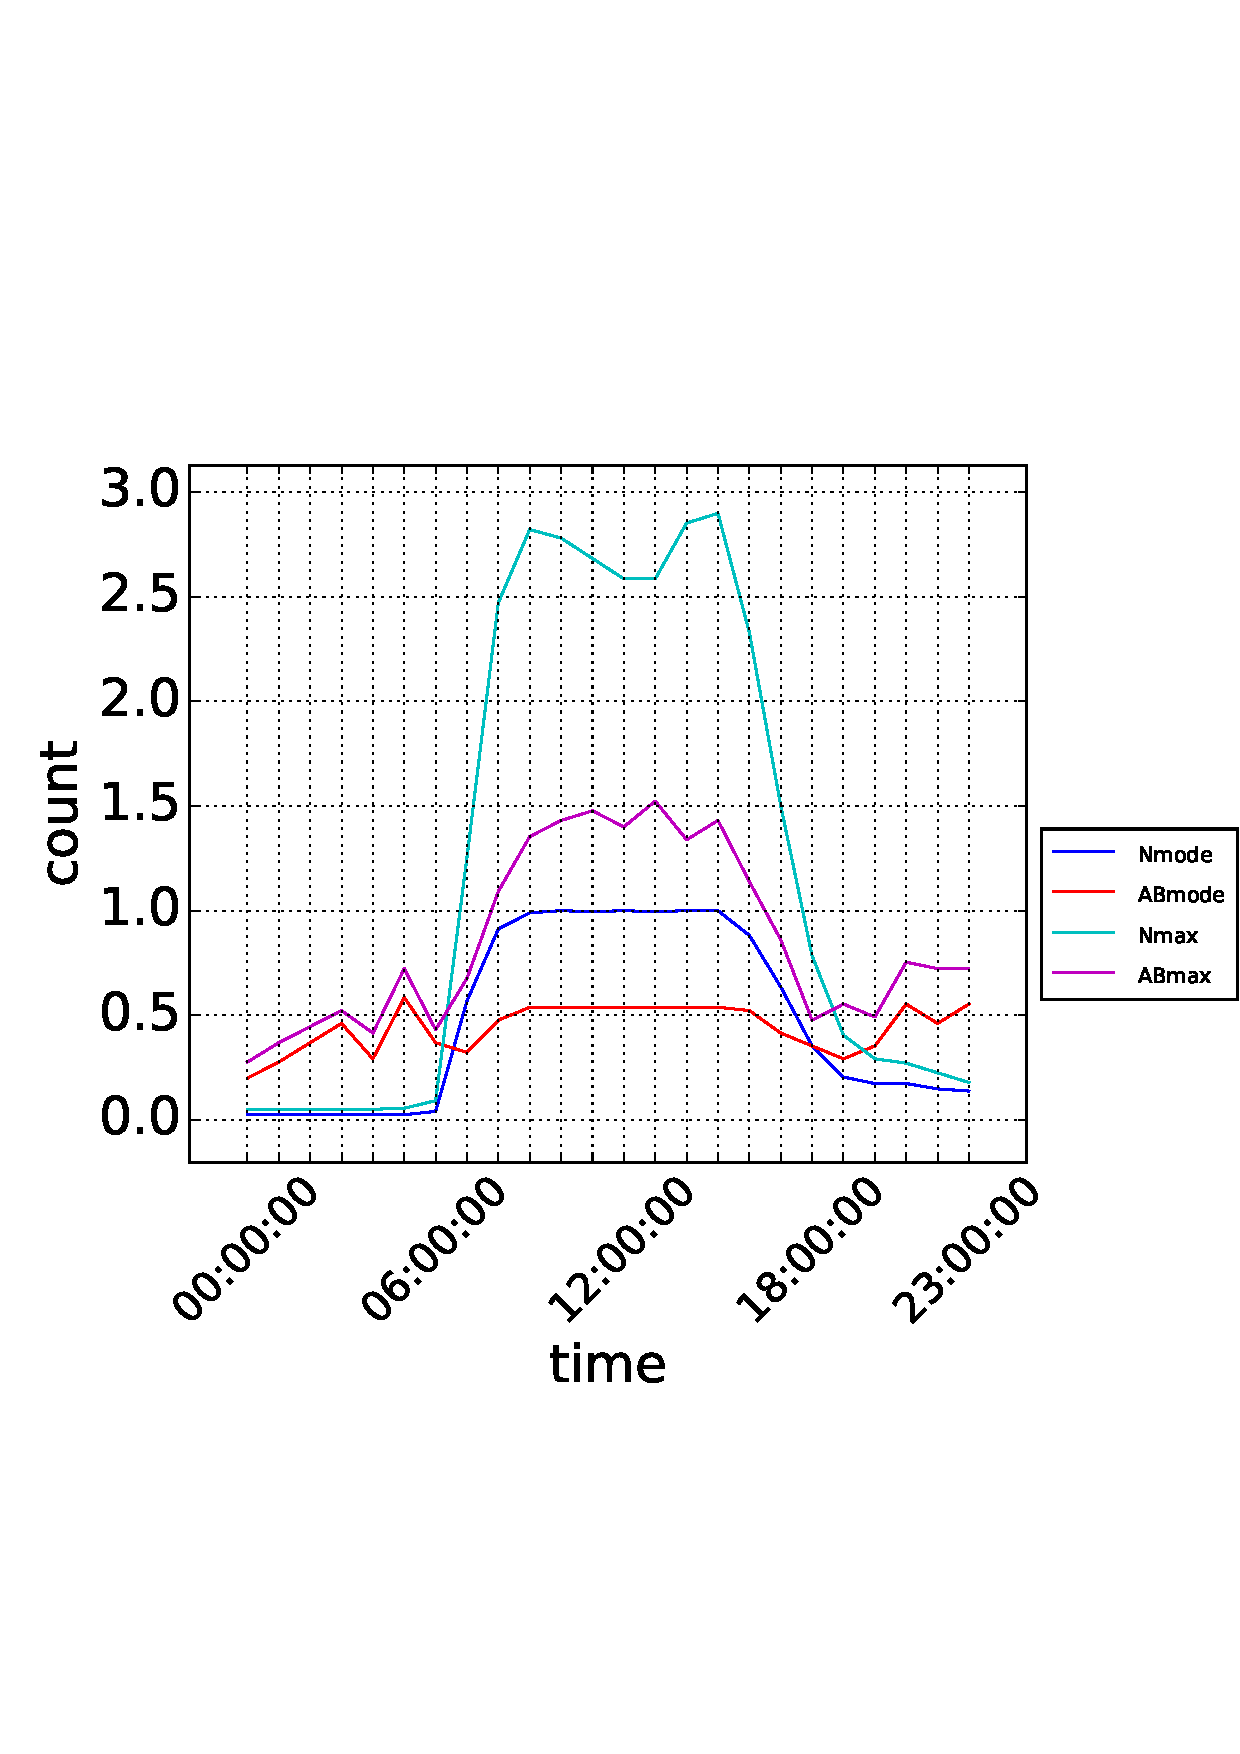
\includegraphics[width=2.8in]{figure/figure53.png}
}
\caption{ Removable media usage behavior }
\label{fig5}
\end{figure*}

Removable media usage events. Removable media is among the most popular method used in theft of Intellectual Property (IP) in extracting confidential information from organizations \cite{b41}. Tracking the use of removable media can be an excellent information source for identifying suspicious events by trusted insiders . Baseline behavior of removable media usage is captured by the minimum, maximum, mean and mode time of “Insert” and “Remove” activities as in the logon/logoff event analysis. Time gap between consecutive “Insert - Remove” action has also been identified as a good source of information to capture large file downloads. The daily number of files copied by an individual is also used in this analysis.

For better known about the differences of behavior between normal users and abnormal users at each time, we use the data set which include 930 normal employees and 70 abnormal employees to count their behavior feature separately over a 17 months period. The figure3 show the result.

Individual Logon-Logoff Behavior. Figure 3(a) is an illustration of users logon behavior for the
entire period of the dataset. By looking at this graph, it is evident that the majority of logon activities occur during early office hours, which can be interpreted as the first logon event of the day. This phenomenon applies to everyone.  The logon times which we need to pay more attention are the events which happen during after office hours. We can identify abnormal users who have maximum logon times occurred during the late night, which indeed is unusual for normal operations. One of the other critical parameters of insider threat detection, the “logoff” behavior of users are illustrated in Figure 3(b). This graph also shows the mode and maximum logoff times of each user for the entire period. As can be seen on the graph majority of “logoff” events happen during late office hours for normal users. For abnormal users, the times increased significantly of logoff behavior. they are more active during after office hours.

Removable media usage. Figure 4 is an illustration of users’ removable media usage statistics.
Similar to logon/logoff analysis, time dependencies of removable media usage has also been investigated. Figure 4(a) and (b) shows the maximum and mode times for USB connect and disconnect events respectively. We can find that the maximum of times for USB connect and disconnect events of the normal user are generally higher than the abnormal user, which can be understood as the need of some jobs. But the times of the behavior frequently occurrences in the morning 0:00 and 6:00, in which  there almost no operation for the normal user.  Abnormal users have a greater probability of abnormal behavior during the period, for example, copy the company internal documents.

Figure 4(c) demonstrate the variation of users daily number of file accesses. To identify suspicious file copies we have considered the maximum and mode of the number of file copies per day by an individual. From the illustration, the normal are more inclined to carry out the operation of the file in the middle of the night compared with the normal.

In summary, we found that there is a a big difference in behavior between normal user and abnormal user at different times, so we decide to merge the times of behavior every 6 hours as the parameter to input to our ADAD model. Figure 5 is an illustration of the parameters.



\begin{table}[tbp]
\caption{Selected parameter set.}
\centering  % 表居中
\begin{tabular}{lc}  % {lccc} 表示各列元素对齐方式,left-l,right-r,center-c
\hline
Module	&Parameter\\ \hline
	
Logon events	& \tabincell{c}{Maximum/Mode Alogon counts(00:00-06:00)\\Maximum/Mode Blogon counts(06:00-12:00)\\Maximum/Mode Clogon counts(12:00-18:00)\\Maximum/Mode Dlogon counts(18:00-24:00)}\\\hline

Logoff events	& \tabincell{c}{Maximum/Mode Alogoff counts(00:00-06:00)\\Maximum/Mode Blogoff counts(06:00-12:00)\\Maximum/Mode Clogoff counts(12:00-18:00)\\Maximum/Mode Dlogoff counts(18:00-24:00)}\\\hline

Removable Media	& \tabincell{c}{Maximum/Mode Aconnect counts(00:00-06:00)\\Maximum/Mode Bconnect counts(06:00-12:00)\\Maximum/Mode Cconnect counts(12:00-18:00)\\Maximum/Mode Dconnect counts(18:00-24:00)\\Maximum/Mode Adisconnect counts(00:00-06:00)\\Maximum/Mode Bdisconnect counts(06:00-12:00)\\Maximum/Mode Cdisconnect counts(12:00-18:00)\\Maximum/Mode Ddisconnect counts(18:00-24:00)}\\\hline

File copy events	& \tabincell{c}{Maximum/Mode Afilecopy counts(00:00-06:00)\\Maximum/Mode Bfilecopy counts(06:00-12:00)\\Maximum/Mode Cfilecopy counts(12:00-18:00)\\Maximum/Mode Dfilecopy counts(18:00-24:00)}\\\hline

\end{tabular}

\end{table}


After the experiment we found that the features we extracted had noise effects (which in detail in the experimental part), in order to achieve higher accuracy, we use PCA\cite{b42} for denoising. All feature columns are normalized before the PCA decomposition is performed. By default, we consider a decomposition of the features to a 2-D space.

\subsubsection{Anomaly Detection}

Due to the complex nature of insider threat problem, it is extremely hard to pinpoint a user as a malicious insider. Therefore, the first step should be the identification of possible malicious insiders who are maximally deviating from peers as well as their normal behavior. Therefore, as the second stage of our analysis, we will focus on implementing an anomaly detection algorithm based on the the  properties identified at the previous stage of this analysis. The anomaly detection algorithm adopted in this analysis is the “Isolation forest” algorithm, which stands out in effectively separating anomalous events from the rest of the instances \cite{b43}.

Isolation Forest Algorithm - iForest: The isolation forest algorithm is a model-based approach which
explicitly isolates anomalies without constructing a typical profile instance. Linear time complexity with a low constant and low memory requirements drives us to use it in our experiments as the enormous amount of information need to be analyzed in the field of insider threat. The use of the isolation forest algorithm for this work is part of the overall research effort within our research group at RMIT University and CA Pacific, with the details as presented in \cite{b44}, where it is applied to a very large enterprise system for anomaly detection. This algorithm also performs well with a large number of irrelevant attributes and instances where training data set does not contain any anomalies. This method generates an ensemble of iTrees for a given dataset and the instances with the short average path of iTrees are considered to be anomalies. If the calculated anomaly score value, s is very close to 1 it can be regarded as a definite anomaly. Instances with s much smaller than 0.5 can be considered normal situations. If all the instances return s ≈ (0.5), then the entire sample deemed to be not having any distinct anomalies.


\subsection{Approach 2: Across-Time Anomaly Detection(ATAD)}

We note that while a particular activity may not be suspicious, a rare change in activity can be. In this section we use Markov chain model \cite{b45} to detects individuals with unusual changes in activity. Figure 6 shows a graphical overview of the processing approach and pipeline we use, and the remainder of this section is dedicated to describing each stage in it.

\begin{figure}[htb]
\centerline{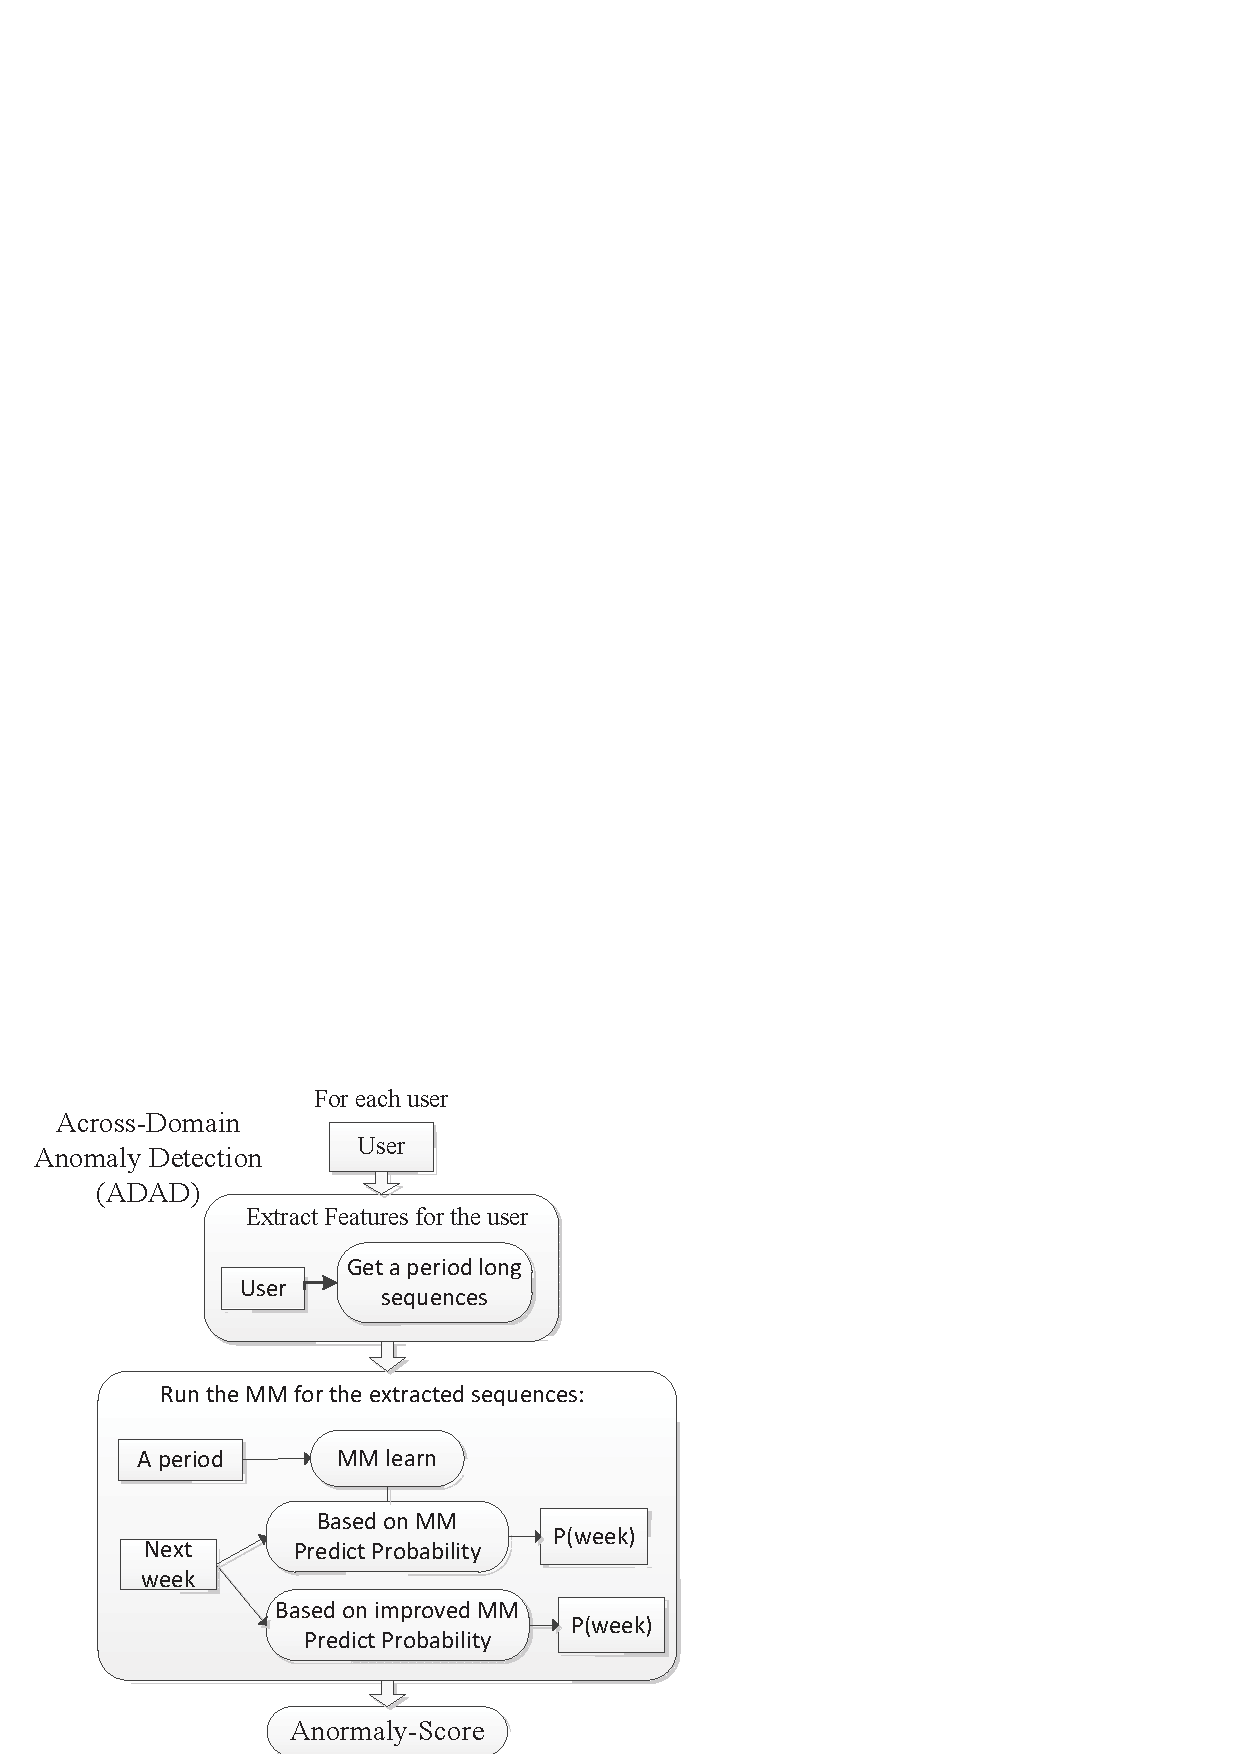
\includegraphics[width = 0.8\textwidth]{figure/figure6.png}}
\caption{An overview of the Across-Time Anomaly Detection(ATAD).}
\label{fig}
\end{figure}
\subsubsection{Feature Extraction}

The CERT Dataset contains many log files which describe a particular kind of activity for all users (users being the same as employees), for instance http.csv contains logs pertaining to web browsing (website, date accessed, username, etc.). We load each file, and assign a symbol to each entry based on the set of features we are defined in ADAD. For example, if a user logon between 00:00 and 06:00,we define this activity as “ALogon”, between 06:00 and 12:00,we define it as “BLogon”, between 12:00 and 18:00,we define it as “CLogon”, between 18:00 and 24:00,we define it as “DLogon”, and we treat them as different behaviors. After this, we join all of these files, partition them by each user and then finally sort them based on the respective timestamps. For each user we get a list of actions and the time at which they undertook them.

We then group these actions into two parts,one is the action in last week,the other is the rest of the time, which gives us the final output for the feature extraction phase. for each part we have a sequence of actions the user took. Experimenting with the time-scale we use is an interesting avenue of research that we have not explored in this paper, but reserve for future study. We should note that the CERT Dataset contains the ground truth for each user (when they are acting maliciously or not), which allows us to monitor the success or failure of our experiment.

\subsubsection{Anomaly Detection}

Once we have a sequence of actions that each user conducted in a period, we are able to use our Markov Model (MM)\cite{b46}. Here, behaviors correspond to model states. Let P$_{ij}$ denote the probability that the user is in a state j at time t+1 given the user is in state t at time t.The probability that a sequence of states X$_1$, … , X$_T$ at time 1, … , T occurs in the context of the stationary Markov chain is computed as follows:
\begin{align}
P(X_1,...,X_T)=q_{x1}\sum_{t=2}^T P_{X_{t-1}X_t}
\end{align}



\iffalse
 we has a finite number of states, 1, 2, … , s, the stationary Markov chain can be defined by a transition probability matrix \cite{b46}:


$$p=\begin{bmatrix}
p_{11}&p_{12}&...&p_{1s}\\
p_{21}&p_{21}&...&p_{2s}\\
.&.&.&.\\
.&.&.&.\\
.&.&.&.\\
p_{s1}&p_{s2}&...&p_{ss}
\end{bmatrix}$$

and an initial probability distribution\cite{b46}:


$$p=\begin{bmatrix}
q_{1}&q_{2}&...&q_{s}
\end{bmatrix}$$


where q$_{i}$ is the probability that the system is in state i at time 0, and

$$\sum_{j=1}^{j=s} p_{ij}=1$$

The probability that a sequence of states X$_1$, … , X$_T$ at time 1, … , T occurs in the context of the stationary Markov chain is computed as follows:

$$P(X_1,...,X_T)=q_{x1}\sum_{t=2}^T P_{X_{t-1}X_t}$$

The transition probability matrix and the initial probability distribution of a stationary Markov chain can be learned from the observations of the system
state in the past. Provided with the observations of the system state X$_0$, X$_1$, X$_2$, … , X$_N-1$ at time t = 0, … , N-1, we learn the transition probability matrix and the initial probability distribution as follows \cite{b47}:

$$p_{ij}=N_{ij}/N_i$$
$$q_i=N_i/N$$

where
\begin{itemize}
\item N$_{ij}$ is the number of observation pairs X$_t$ and X$_t+1$ with
\item X$_t$ in state i and X$_t+1$ in state j;
\item N$_i$. is the number of observation pairs Xt and Xt+1 with
\item X$_t$ in state i and X$_t+1$ in any one of the states 1, … , s;
\item N$_i$ is the number of X$_t$’s in state i; and
\item N is the total number of observations.
\end{itemize}
\fi

Individuals are scored based on their total transition likelihood over time, and suspicious individuals with unusual transitions between temporal states are detected. We use three methods to get the user’s score of last week to compare detection one based on MM and the other based on improved MM.

Baesd on MM:
\begin{align}
R_{score} = P(X_1,...,X_T)
\end{align}


Based on improved MM:

Firstly,We treat the sequences of the week(X$_1$,X$_2$,......X$_T$) as a whole,the anomaly score R$_{point}$ for the user is calculated by estimating the user’s transition likelihood over time. The anomaly probability score is computed as
\begin{align}
R_{point}=q_{x1}\prod_{t=2}^T P_{X_{t-1}X_t}..
\end{align}

Secondly,we regard the sequences of every day during this week (X$_{11}$,X$_{12}$,......X$_{WT}$)as a whole and treat the average daily anomaly score as the anomaly score of the week named R$_{trend}$ computed as 
\begin{align}
R_{trend}=1/w\sum_{t=1}^W {q_{x1}\prod_{t=2}^T P_{X_{w(t-1)}X_wt}}
\end{align}


\subsection{Information fusion for combining anomaly indicators}

Our goal is to combine suspicion/anomaly scores that have been generated from each of the aforementioned methods to detect anomalies. We note that in a more general analytics framework, the same technique can be used to combine scores based on relative importance or surprise/risk levels.

In anomaly detection, an individual can be anomalous in one domain or at a time instance. Also, the relative suspicion of an individual can vary from one indicator (or information source) to another. However, most anomaly detection applications require a single overall conclusion about the relative suspicion of each individual. Therefore, we developed a technique based on weight fusion to combine multiple sources and time-series of evidence from multiple domains. In a broad sense, each source of information provides a suspicion score and the goal is to combine these scores in order to identify anomalies with greater accuracy. We combine the predictability score of multi-domain and time-series instance to compute a single, combined suspicion score for each user to identify the anomalous individuals.The combined suspicion score is computed as

\begin{align}
R_{combined}&= W_1*R_{ADAD}+W_2*R_{ATAD}\\
r&=\begin{cases}
w_2/w_1
&\mbox{if } w_1 \textgreater 0\\
1
&\mbox{if } w_1 \equiv 0\\
\end{cases}
\end{align}


\section{Experiment Results}

This section is dedicated to a comprehensive discussion of results obtained through our analysis.

\subsection{Across-Domain Anomaly Detection(ADAD)}\label{AA}

Figure 7 shows the results of running our model ADAD with those parameters. Firstly, we treat the feature of every domain as the input to detect separately, then we input features of all domain to detect. We found that removable media domains is the most predictable (with the highest predictive accuracy), while Logon and file domains are harder to predict. It appears that users show great variation in their logon and file behavior, but are more uniform in device usage . Except that, the property of the mode is more effective than maximum to detect, which indicates that the mode  represents the difference between normal and abnormal. Finally, we use PCA to decompose of the features to a 2-D space,and get a higher predictive accuracy.


\begin{table}[tbp]
\caption{The experiment result of ADAD.}
\centering  % 表居中
\begin{tabular}{lcccc}  % {lccc} 表示各列元素对齐方式,left-l,right-r,center-c
\hline
iForest Input & 	&Accurate &Precision &Recall\\ \hline
	
Logon 	& MAX &89\% &32\% &47\%\\
  & MODE &87\% &22\% &34\%\\\hline
Logoff 	& MAX &88\% &23\% &34\%\\
   & MODE &85\% &14\% &21\%\\\hline
Connet 	& MAX &78\% &65\% &27\%\\
  & MODE &79\% &70\% &28\%\\\hline
Disconnect 	& MAX &80\% &73\% &30\%\\
  & MODE &79\% &69\% &28\%\\\hline
Filecopy 	& MAX &80\% &60\% &28\%\\
  & MODE &77\% &44\% &20\%\\\hline
All properties 	& MAX &82\% &68\% &34\%\\
  & MODE &79\% &52\% &31\%\\\hline
All properties 	& dimension=2 &87\% &79\% &35\%\\\hline

\end{tabular}

\end{table}


\subsection{Across-Time Anomaly Detection(ATAD)}


We apply our Across-Time Anomaly Detection(ATAD) detection method as follows. It's obvious that the improved MM method is more effective than the mathod based on MM. For improved MM,the impro\_Point(iP) is the experience that the week is a whole. The impro\_Trend(iT) is the experience that the day is a whole, based on which we regard the average of this week's daily anomaly score as the final anomaly score of the week. Compare with the iP, iT has a better result. This is because that for  iP if a user has once unusual change during this week,which will has a important influence on the final result,maybe the change just is working overtime. This will has effect on the detection. However, it can avoid the miscarriage of justice brought about by this accidental abnormal changes to some extent for  iT. In other words,  iT is more likely to detect abnormal changes in behavioral trends over a period of time, which detect insider threat more accurately. And we will regard AAS as the result of ATAD to combine with ADAD in next section.

\begin{figure}[htb]
\centerline{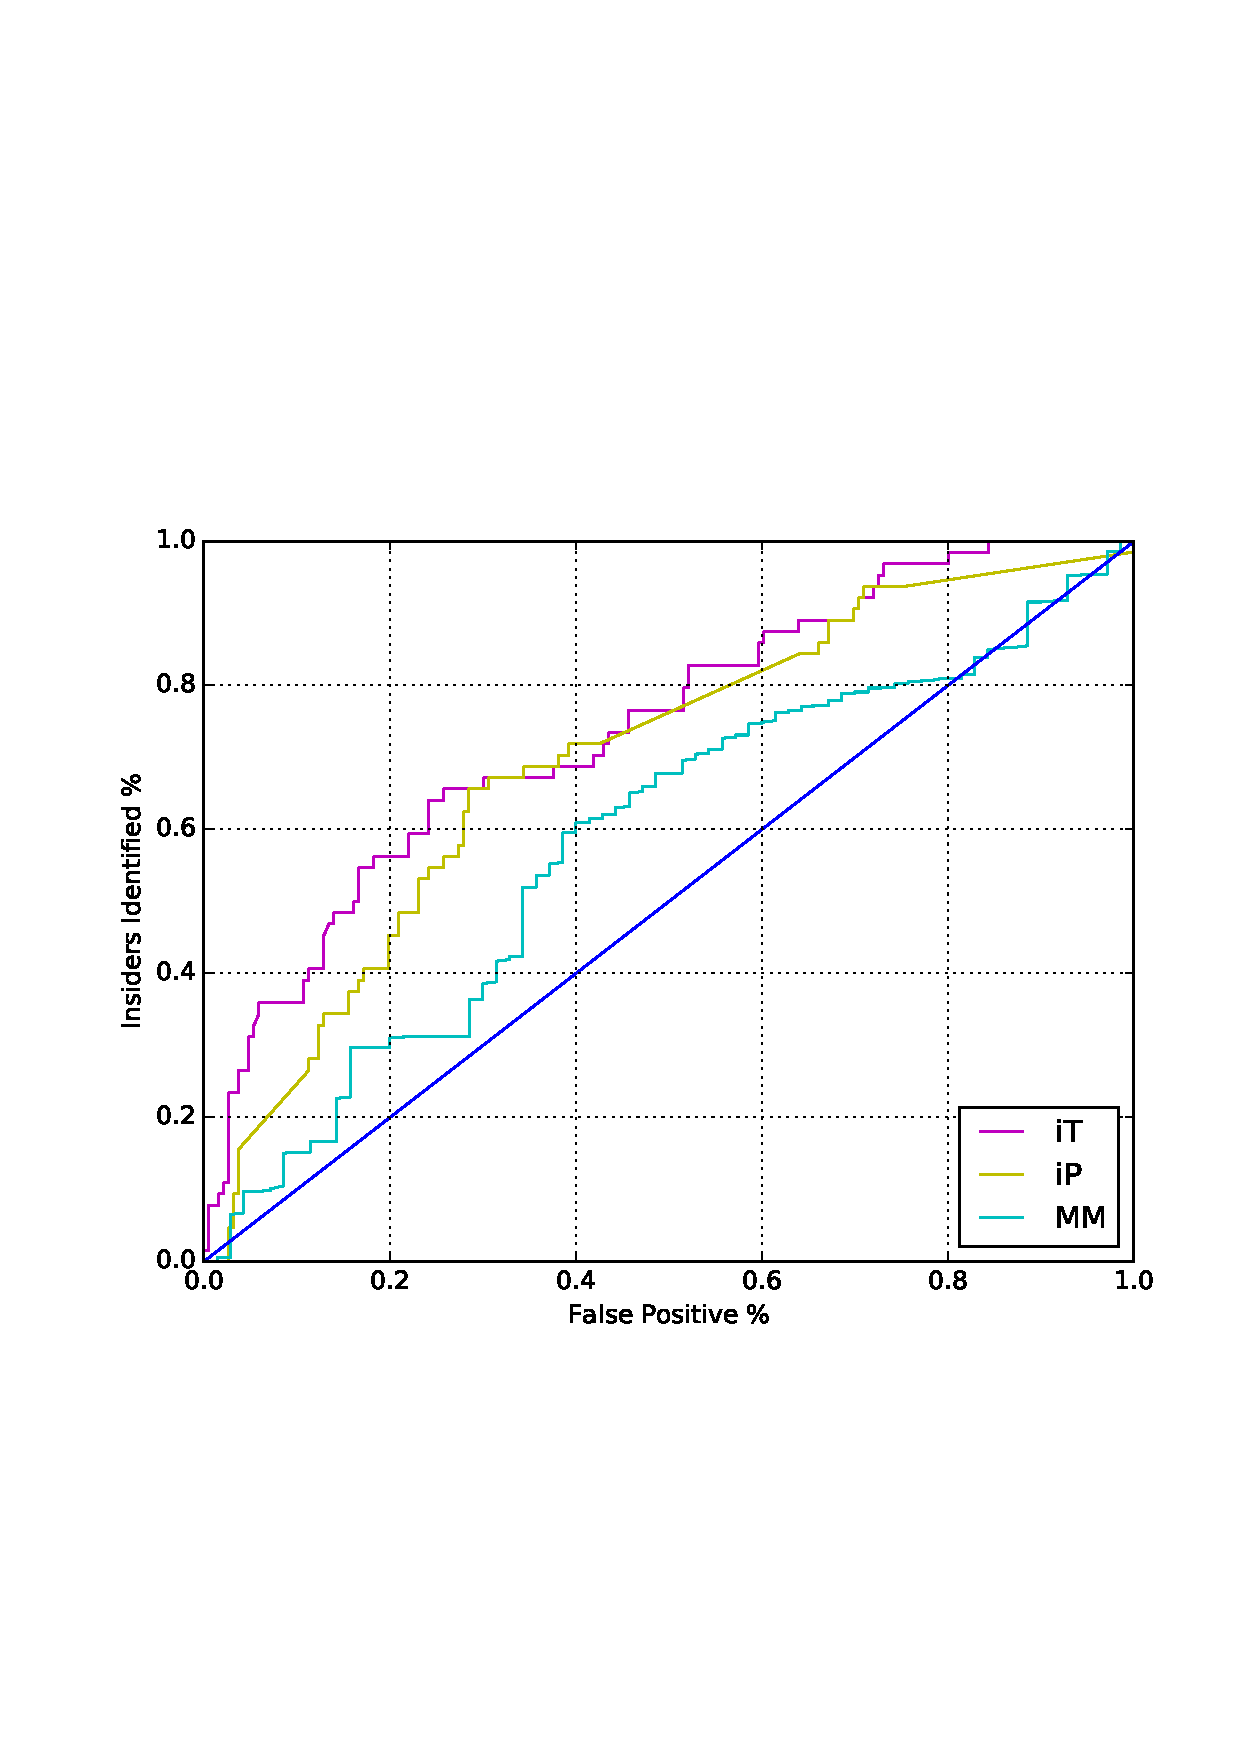
\includegraphics[width = 0.5\textwidth]{figure/figure7.png}}
\caption{ROC Curve showing the differences between MM algorithm and improved MM algorithm.}
\label{fig}
\end{figure}


\subsection{Information fusion for combining anomaly indicators}

We get the final anomaly score based on weight fusion as shown in Table 2. r represents the proportion of the weight of the two methods score. The scores are normalized before the weight fusion(combine).When r = 0, it is the result of individual ADAD method, when r = 1, it is the result of individual ATAD method. We can see that when r is 3/7, the accuracy and recall rate is the highest, where the combination of weights is the best. Indeed, it is remarkable that a suitable combination of the individual ATAD and ADAD scores in an appropriate fashion leads to significant improvement in performance relative to any of the individual ATAD or ADAD sources.


\begin{table}[tbp]
\caption{The experiment result of information fusion.}
\centering  % 表居中
\begin{tabular}{lcc}  % {lccc} 表示各列元素对齐方式,left-l,right-r,center-c
\hline
r  &Precision &Recall\\ \hline
0(ADAD) &79.17\% &35.19 \\\hline
1/9 &90\% &35.18\%\\\hline
2/8 &94.44\% &31.48\%\\\hline
3/7 &95\% &35.19\%\\\hline
4/6 &74.73\% &33.33\% \\\hline
5/5 &90\% &33.33\% \\\hline
6/4 &85\% &31.48\%\\\hline
7/3 &82.35\% &25.92\%\\\hline
8/2 &66.67\% &25.92\%\\\hline
9/1 &61.9\% &24.07\%\\\hline
1(ATAD) &60\% &27.78\%\\\hline
\end{tabular}

\end{table}

Figure 8 is an indication of how the anomaly scores are distributed when r is 3/7 in this analysis. The graph indicated few points above the “Red” color horizontal line which is equivalent to an anomaly score of 1.3. Users belong to those points can be considered as anomalous users.To get a better understanding and visualization of results based on our approach, we mark the positive sample with red and negative sample with blue. It indicates that 95 percent of the insider threaters we detected are true insider threaters.  

\begin{figure}[htb]
\centerline{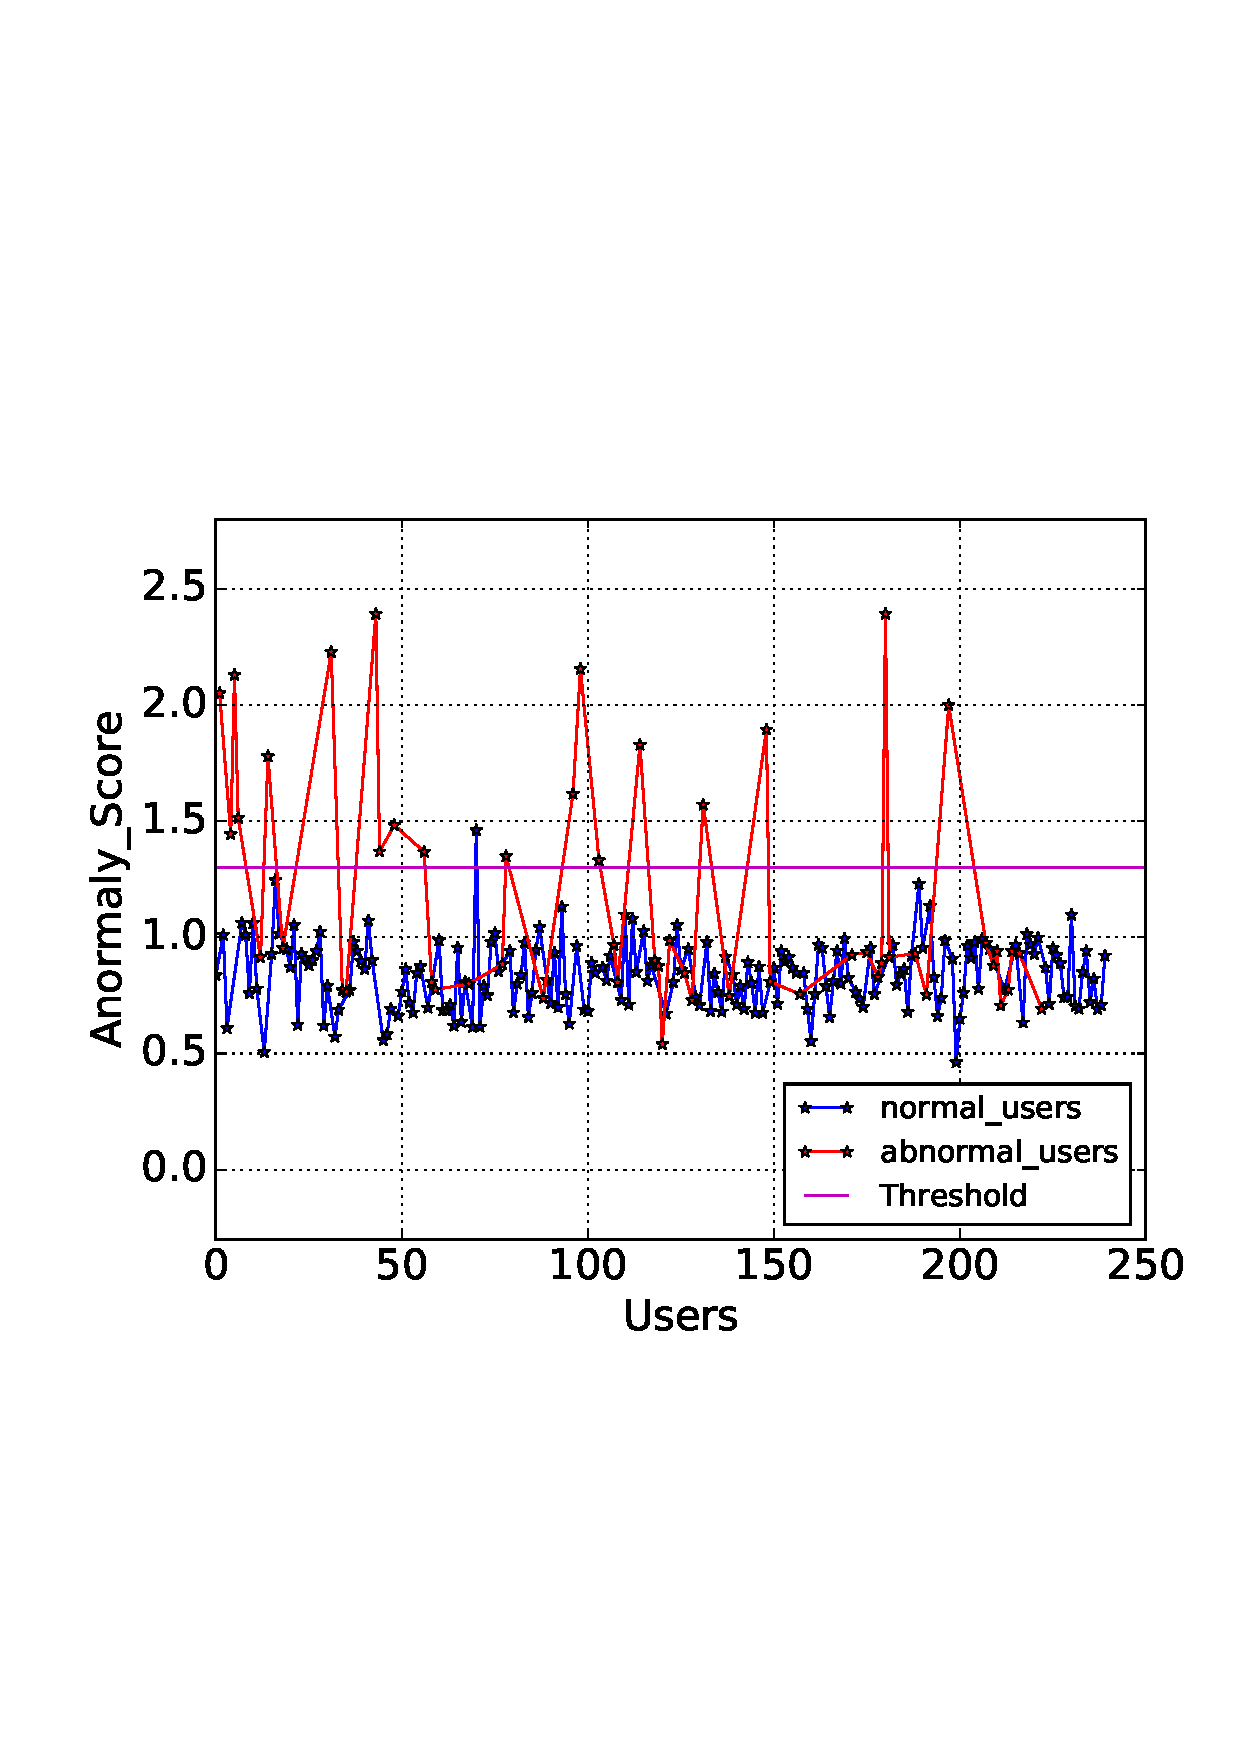
\includegraphics[width = 0.5\textwidth]{figure/figure8.png}}
\caption{Anomaly score distribution.}
\label{fig}
\end{figure}

\section{Conclusion}

In this paper we have examined the problem of insider threat detection. Our main contribution is that a novel fusion approach for robust detection of anomalies is discussed. The two main components of our framework - ADAD and ATAD - improve anomaly detection prediction accuracy by combining information from multiple domains and time-instances.As a result, these methods are able to determine anomalies that not only act inconsistent with peers but also has unusual change compared with their historic action. 

Previous anomaly detection methods for work practice data treated each domain separately.  The ADAD improves prediction accuracy by combining information from multiple domains, The main novelty of our proposed method is that it combines model information from each domain, rather than only anomaly scores from each domain.  The ATAD allows us to visualise the model, and thus to determine what the model deems as normal behaviour which allows us to understand why a particular sequence of actions is classified as anomalous. This is extremely pertinent information, since there are severe repercussions when an employee is flagged as a potential threat to an organisation. 

Based on this, we have proposed a effective method based on weight combination to fuse the results generated from ADAD and ATAD . Our fusion scheme offers the advantage of being robust to variance in the individual outputs of MDCV and CD while combining their information in order to improve the quality of anomaly detection. We verify the improved robustness and accuracy of our proposed algorithm via experimental results on detecting insiders from a large, public data set.

\section{Limitation and future work}

In the exploration into the utility of a Fusion Method based on multi-dimensional features to insider threat detection, we have made many assumptions that could limit the effectiveness of our approach in certain scenarios. We enumerate the most important of these, and the possible effect they could have on our system below.

Insider attacks are anomalous(不是很理解,标题理解,具体内容不懂): The most significant assumption we have made is that all insider attacks are examples of anomalous behaviour. This precludes us from recognising situations where a user systematically attacks an organisation over an extended time-framework (e.g., downloading sensitive files over months), or situations where our features are not sufficient to distinguish an attack from a user’s normal behaviour.

User behavior is almost consistent in ADAD:in ADAD model, We assume that the behavior of all is basically the same, based on which we could identify people who inconsistent with the public. In fact, There are some differences in the behavior of people in different positions, it reserve for future study.

Training on a period data in ATAD: 
In order to apply our ATAD model, we must first ensure that it is able to distinguish a user’s normal behaviour from anomalous behaviour. This then means that we must train on some sample of a user’s behaviour in order for the model to learn normal behaviour. Hence we are not looking for insider threats in that training set, which in our specific case means that we do not consider that a user might attack in a period data. This could significantly hamper our ability to detect insider threats amongst short-term users (contractors for instance), which are a real threat \cite{b48}.

Features: Our approach is only able to make use of the information that it is provided, and hence depends on the features that it is supplied with. This requires domain knowledge and manual feature engineering and experimentation in order to produce useful features. Our approach would therefore need to be adapted somewhat depending on application cases.

\subsection{Future work} 
Threshold:Our current procedure for determining if the anomaly score is anomalous or not is to compare with a threshold. This requires us to manually set a threshold value, which is another hyperparameter of our system that significantly affects the results. However, we could consider the task of determining which score is anomalous as an anomaly detection problem itself. Hence, we could apply a novel outlier threshold selection algorithm that aids in analyzing the specific domain and time-instance related events that were responsible for a particular to be flagged with a high anomaly rank.(e.g., \cite{b49}) on the anomaly score generated by our model. This allows us to avoid having to manually set a threshold parameter.

Fusion method \&\& Recall \&\& Role\_based	:We use a combined method based on weight fusion to integrate the ADAD and the ATAD, which has a high precision but a pessimistic recall. To solve this problem, we could apply on some complex and effective fusion scheme to combine their information in order to improve the recall of anomaly detection(e.g.,\cite{b49}).  In addition, we could take user role into account in generates user Normal portrait that can describe the full extent of activities that users perform within the organization based on role to improve the recall of anomaly detection(e.g.,\cite{b50}).   	


\section*{Acknowledgment}

The preferred spelling of the word ``acknowledgment'' in America is without 
an ``e'' after the ``g''. Avoid the stilted expression ``one of us (R. B. 
G.) thanks $\ldots$''. Instead, try ``R. B. G. thanks$\ldots$''. Put sponsor 
acknowledgments in the unnumbered footnote on the first page.



\begin{thebibliography}{00}
\bibitem{b1}A. M. Dawn Cappelli Randall Trzeciak,Timothy J. Shimeall,“Common Sense Guide to Prevention and Detection of Insider
Threats , 3rd Edition,” 2009.
\bibitem{b2} Gemalto. Breach level index|data breach database \& risk assessment calculator, 2016. http://www.breachlevelindex.com/.
\bibitem{b3} “By the numbers: Cyber attack costs compared,” 2016, accessed on 31/05/2016. [Online]. Available: http://www.csoonline.com/article/3074826/security/bythe-numbers-cyber-attack-costs-compared.html
\bibitem{b4} Teresa F Lunt. A survey of intrusion detection techniques. Computers \& Security, 12(4):405–418, 1993.
\bibitem{b5} Sunu Mathew, Michalis Petropoulos, Hung Q Ngo, and Shambhu Upadhyaya. A data-centric approach to insider attack detection in database systems. In Recent Advances in Intrusion Detection, pages 382–401. Springer, 2010.
\bibitem{b6} William Eberle, Jeffrey Graves, and Lawrence Holder. Insider threat detection using a graph-based approach. Journal of Applied Security Research, 6(1):32–81, 2010.

\bibitem{b7} Alex Memory, Henry G Goldberg, and E Ted. Context-aware insider threat detection. In Workshops at the Twenty-Seventh AAAI Conference on Artificial
Intelligence, 2013.
\bibitem{b8} Robert F Mills, Michael R Grimaila, Gilbert L Peterson, and Jonathan W Butts. A scenario-based approach to mitigating the insider threat. Technical report, DTIC Document, 2011.
\bibitem{b9}  D. Cappelli, A. Moore, and R. Trzeciak, The CERT Guide to Insider Threats: How to Prevent, Detect, and Respond
to Information Technology Crimes (Theft, Sabotage, Fraud). Addison-Wesley Professional, 2012
\bibitem{b10}  Miltiadis Kandias, Alexios Mylonas, Nikos Virvilis, Marianthi Theoharidou, and Dimitris Gritzalis. An insider threat prediction model. In Trust, privacy and security in digital business, pages 26–37. Springer, 2010.
\bibitem{b11}Frank L Greitzer, Lars J Kangas, Christine F Noonan,and Angela C Dalton. Identifying at-risk employees: A behavioral model for predicting potential insider threats. Pacific Northwest National Laboratory Richland, WA, 2010
\bibitem{b12}GB Magklaras and SM Furnell. Insider threat prediction tool: Evaluating the probability of it misuse. Computers \& Security, 21(1):62–73, 2001.
\bibitem{b13}Hoda Eldardiry, Evgeniy Bart, Juan Liu, John Hanley, Bob Price, and Oliver Brdiczka. Multi-domain information fusion for insider threat detection. In Security and Privacy Workshops (SPW), 2013 IEEE, pages 45–51. IEEE, 2013.
\bibitem{b14}Automated Insider Threat Detection System Using User and Role-Based Profile Assessment Philip A. Legg, Oliver Buckley, Michael Goldsmith, and Sadie Creese
\bibitem{b15}  Deep Learning for Unsupervised Insider Threat Detection in Structured Cybersecurity Data Streams Aaron Tuor and Samuel Kaplan and Brian Hutchinson∗
Western Washington University Bellingham, WA Nicole Nichols and Sean Robinson Pacific Northwest National Laboratory Seattle, WA
\bibitem{b16}  P. A. Legg et al., “Towards a conceptual model and reasoning structure for insider threat detection,” J. Wireless Mobile Netw., Ubiquitous Comput., Dependable Appl., vol. 4, no. 4, pp. 20–37, Dec. 2013.
\bibitem{b17} M. Bishop et al., “Insider threat detection by process analysis,” in Proc. IEEE SPW, 2014, pp. 251–264.
\bibitem{b18}] M. Bishop, S. Engle, S. Peisert, S. Whalen, and C. Gates, “We have met the enemy and he is us,” in Proc. NSPW, Lake Tahoe, CA, USA, Sep. 2008, pp. 1–12
\bibitem{b19} J. R. C. Nurse et al., “Understanding insider threat: A framework for characterising attacks,” in Proc. IEEE SPW, 2014, pp. 214–228
\bibitem{b20}F. Kammueller and C. W. Probst, “Invalidating policies using structural information,” J. Wireless Mobile Netw., Ubiquitous Comput., Dependable Appl., vol. 5, no. 2, pp. 59–79, Jun. 2014.
\bibitem{b21} M. R. Ogiela and U. Ogiela, “Linguistic protocols for secure information management and sharing,” Comput. Math. Appl., vol. 63, no. 2, pp. 564–572, Jan. 2012.
\bibitem{b22}G. B. Magklaras and S. M. Furnell, “Insider threat prediction tool: Evaluating the probability of IT misuse,” Comput. Security, vol. 21, no. 1, pp. 62–73, 1st Quart. 2002.
\bibitem{b23} L. Spitzner, “Honeypots: Catching the insider threat,” in Proc. 19th IEEE ACSAC, Las Vegas, NV, USA, Dec. 2003, pp. 170–179.
\bibitem{b24}G. B. Magklaras and S. M. Furnell, “Insider threat prediction tool: Evaluating the probability of IT misuse,” Comput. Security, vol. 21, no. 1, pp. 62–73, 1st Quart. 2002.
\bibitem{b25} J. Myers, M. R. Grimaila, and R. F. Mills, “Towards insider threat detection using web server logs,” in Proc. 5th Annu. CSIIRW—Cyber Security Inf. Intell. Challenges Strategies, New York, NY, USA, 2009, pp. 54:1–54:4.
\bibitem{b26} M. A. Maloof and G. D. Stephens, “Elicit: A system for detecting insiders who violate need-to-know,” in Recent Advances in Intrusion Detection, vol. 4637, Lecture Notes in Computer Science, C. Kruegel, R. Lippmann, and A. Clark, Eds. Berlin, Germany: Springer-Verlag, 2007, pp. 146–166.
\bibitem{b27} J. S. Okolica, G. L. Peterson, and R. F. Mills, “Using PLSI-U to detect insider threats by datamining e-mail,” Int. J. Security Netw., vol. 3, no. 2, pp. 114–121, 2008.
\bibitem{b28}Y. Liu et al., “SIDD: A framework for detecting sensitive data exfiltration sby an insider attack,” in Proc. 42nd HICSS, Jan. 2009, pp. 1–10.
\bibitem{b29} H. Eldardiry et al., “Multi-domain information fusion for insider threat detection,” in Proc. IEEE SPW, May 2013, pp. 45–51.
\bibitem{b30} Brdiczka et al., “Proactive insider threat detection through graph learning and psychological context,” in Proc. IEEE Symp. SPW, San Francisco, CA, USA, May 2012, pp. 142–149.
\bibitem{b31}W. Eberle, J. Graves, and L. Holder, “Insider threat detection using a graph-based approach,” J. Appl. Security Res., vol. 6, no. 1, pp. 32–81, Dec. 2010.
\bibitem{b32}B. Klimt and Y. Yang, “The enron corpus: A new dataset for email classification research,” in Machine Learning: ECML 2004, vol. 3201, Lecture Notes in Computer Science, J.-F. Boulicaut, F. Esposito, F. Giannotti, and D. Pedreschi, Eds. Berlin, Germany: Springer-Verlag, 2004, pp. 217–226
\bibitem{b33}T. E. Senator et al., “Detecting insider threats in a real corporate database of computer usage activity,” in Proc. 19th ACM SIGKDD Int. Conf. Knowl. Discov. Data Mining, 2013, pp. 1393–1401.
\bibitem{b34}P. Parveen, J. Evans, B. Thuraisingham, K. W. Hamlen, and L. Khan, “Insider threat detection using stream mining and graph mining,” in Proc. IEEE 3rd Int. Conf. Social Comput. PASSAT, Oct. 2011, pp. 1102–1110.
\bibitem{b35}P. Parveen and B. Thuraisingham, “Unsupervised incremental sequence learning for insider threat detection,” in Proc. IEEE Int. Conf. ISI, Jun. 2012, pp. 141–143.
\bibitem{b36}S. Greenberg, Using unix: Collected traces of 168 users, Univ. Calgary, Calgary, AB, Canada, Tech. Rep., 1988.
\bibitem{b37}A New Take on Detecting Insider Threats: Exploring the use of Hidden Markov Models
\bibitem{b38}Automated Insider Threat Detection System Using User and Role-Based Profile Assessment Philip A. Legg, Oliver Buckley, Michael Goldsmith, and Sadie Creese
\bibitem{b39}“CERT Insider Threat Data Set,” Software Engineering Institute, Carnegie Mellon University, CERT Division and Exact
Data LLC. [Online]. Available: https://www.cert.org/insiderthreat/tools/
\bibitem{b40}D. Cappelli, A. Moore, and R. Trzeciak, The CERT Guide to Insider Threats: How to Prevent, Detect, and Respond
to Information Technology Crimes (Theft, Sabotage, Fraud). Addison-Wesley Professional, 2012.
\bibitem{b41} D. Cappelli, A. Moore, and R. Trzeciak, The CERT Guide to Insider Threats: How to Prevent, Detect, and Respond
to Information Technology Crimes (Theft, Sabotage, Fraud). Addison-Wesley Professional, 2012.
\bibitem{b42}I. Jolliffe, Principal Component Analysis. Hoboken, NJ, USA: Wiley,2005.
\bibitem{b43}F. T. Liu, K. M. Ting, and Z. H. Zhou, “Isolation forest,” in 2008 Eighth IEEE International Conference on Data Mining,
Dec 2008, pp. 413–422
\bibitem{b44}L. Sun, S. Versteeg, S. Boztas, and A. Rao, “Detecting anomalous user behaviour using an extended Isolation Forest algorithm: An enterprise case study,” Sept 2016, arXiv:1609.06676.
\bibitem{b45}W. L. Winston, Operations Research: Applications and Algorithms. Belmont, CA: Duxbury Press, 1994.
\bibitem{b46}W. L. Winston, Operations Research: Applications and Algorithms. Belmont, CA: Duxbury Press, 1994.
\bibitem{b47}T. M. Mitchell, Machine Learning. Boston,
MA: McGraw-Hill, 1997.
\bibitem{b48} J. R. C. Nurse, O. Buckley, P. A. Legg, M. Goldsmith, S. Creese, G. R. Wright, and M. Whitty. Understanding insider threat: A framework for characterising attacks. In IEEE Security and Privacy Workshops (SPW). IEEE, 2014. DOI: 10.1109/SPW.2014.38.
\bibitem{b49}Eldardiry H, Sricharan K, Liu J, et al. Multi-source fusion for anomaly detection: using across-domain and across-time peer-group consistency checks[J]. Computing \& Informatics, 2014, 31(3):575-606.
\bibitem{b50} Legg P A, Buckley O, Goldsmith M, et al. Automated Insider Threat Detection System Using User and Role-Based Profile Assessment[J]. IEEE Systems Journal, 2017, 11(2):503-512.






\end{thebibliography}

\end{document}
